\documentclass[journal]{IEEEtran}

\usepackage{blindtext}
\usepackage{graphicx}
\usepackage{cite}
\usepackage[utf8x]{inputenc}
\usepackage[slovene,english]{babel}  
\usepackage{url}

\hyphenation{op-tical net-works semi-conduc-tor}
\begin{document}
\title{IMapBooks - Automatic Question Response Grading}
\author{Tilen Tomakić\\tt5157@student.uni-lj.si\\https://github.com/TilenTomakic/IMapBooks-AQRG\\https://hub.docker.com/r/tilen/sag}%
\maketitle

%  Abstract -  summary of problem and contribution
\begin{abstract}	
  Dokument opisuje raziskavo metod mapiranja, ekstrakcije informacij in uporabe korpusa za točkovanje pravilnosti odgovorov na vprašanja iz podane zgodbe. Uporabljeni so bili tri pristopi (metode). Od osnovnega do naprednejšega.
\end{abstract}

\begin{IEEEkeywords}
NLP, IMapBook, SAG, CAM
\end{IEEEkeywords}

\IEEEpeerreviewmaketitle

% Introduction - problem motivation and background
\section{Uvod}
V angleščini problemsko domeno imenujemo "Short Answer Grading (SAG)". SAG se ukvarja z ocenjevanjem krajših odgovorov (2-3 stavki).

Cilj je bil raziskati tehnike ovrednotenja pravilnosti odgovorov. Pri ovrednotenju je že na voljo množica ovrednotenih odgovorov na enaka vprašanja. Odgovori odgovarjajo na vprašanja podana iz besedila oz. zgodbe.

Problem zaznave pravilih in napačnih odgovorov nam lahko pomaga tudi pri širših problemskih domenah, kot so zaznava lažnih novic.\\

Raziskava je bila osnovana na podatkovni množici vprašanj in odgovor iz IMapBook (\textit{https://www.imapbook.com/}) vira. V množici, sta dva učitelja ovrednotila odgovore učencev na temo prebrane zgodbe. Odgovori so ovrednoteni s 0, 0,5 ali 1 točko.\\

Opisani so tri pristopi reševanja problema. Modeli A, B in C. Enako kot učitelja modeli ovrednotijo odgovore s točkami 0, 0,5 ali 1. Modeli so bili spisani s ciljem neodvisnosti od poznavanja tematike domene, s tem jih je mogoče uporabiti ne le v primeru zgodb.

%  Related work - relevant literature overview
\section{Podobna dela}
Obstaja več strategij oz. kombinacij reševanja problem a ocenjevanja~\cite{adhya2016automated}.
Strategije delimo na slikanje koncepta (angl. concept mapping), ekstrakcija informacij (angl. information extraction), metode s pomočjo korpusov (angl. corpus-based methods), strojno učenje (angl. machine learning) in vrednotenje (angl. evaluation).

Podobni deli temu dokumentu sta CAM (angl. Content Assessment Module)~\cite{bailey2008content} in delo Ulrike Pado in Cornelia Kiefer~\cite{Kiefer}.\\

CAM pristop integrira več strategij ujemanja na različnih stopnjah obdelanega besedila. Na ta način primerja in oceni pomen odgovora.
Na splošno CAM primerja odgovor z znano bazo odgovorov in ugotovi ali odgovor vsebuje enak semantični pomen~\cite{bailey2008diagnosing}.\\

Delo Ulrike Pado in Cornelia z angl. naslovom \textit{Short Answer Grading: When Sorting Helps and When it Doesn’t} je najbolj podobno modeloma B in C opisana v tem dokumentu. Kot glavno komponento sta avtorja uporabila binarno klasifikacijo. Rezultati uspešnosti so primerljivi z ugotovitvami pri C modelu (testna množica IMapBook vprašanja in odgovori).

%  Methods - used methods and techniques
\section{Uporabljene metode}
Uporabljene so bile 3 metode. S ciljem primerjanja izboljšanja rezultatov med njimi. Pričakovano je, da se modela A izkaže kot slaba metoda, model C pa najboljša.

\subsection{Model A}
Model A se že v začetku odloči za en odgovor iz množice vseh pravilnih. Odloči se na podlagi kriterija najpopolnejšega odgovora. Odgovor, ki ima večje število besed se smatra kot najpopolnejši.
Izbran odgovor je uporabljen za ocenjevaje drugih. Bolj sta si odgovora podobna večja je verjetnost, da je ocenjevan odgovor pravilen. Pri primerjanju je odgovor razbit na korene besed.

\subsection{Model B}
Model B je podoben modelu A, vendar se ne odloči za statičen odgovor na začetku. Pravilnost odgovora testira nad celotno znano množico odgovorov.

Ker ima B model na voljo celotno množico odgovor, je bil uporabljena binarna klasifikacija. Poleg žetonov so bili v klasifikaciji upoštevane tudi teme, pridobljene s pomočjo LDA (angl. Latent Dirichlet allocation) algoritma.

\subsection{Model C}
Pri modelu C so za razliko od modela B v klasifikator dodane še sopomenke žetonov. Sopomenke so bile pridobljene s pomočjo uporabe C-net API-ja. Dodatno so bili žetoni spremenjeni v korene besed.

Tu je bil cilj besede poenostaviti na enake imenovalce. Pri prvem poskusu so bili sinonimi direktno dodani v klasifikator. To je povzročilo slabše rezultate, zato sem vse besede, ki imajo enako skupino sinonimov zamenjal le z enim sinonimom (vedno enakim).


% Results - results description
% Discussion - results comparison and evaluation
\section{Rezultati}
Uspešnosti modelov je vidna na tabeli~\ref{t:mod}. V povprečju (F score) se je model C izkazal kot najboljši. Zanimivo je, da ni bil najboljši v vseh skupinah vprašanj. V 3 od 12 primerih je model B dosegel boljšo natančnost. Zato sem kot končno metodo za HTTP strežnik uporabil kombinacijo obeh. Odvisno od vprašanja je bil uporabljen model B ali C, tisti, ki je imel v tej skupini odgovorov na vprašanje boljši povprečni rezultat.

\begin{table}[]
	\begin{tabular}{l|l|l|l|}
		\cline{2-4}
		                            & Model A          & Model B          & Model C          \\ \hline
	
	
	\multicolumn{1}{|l|}{How does Shiranna feel as the shuttle is taking off?} & \textbf{60.49\%} & \textbf{68.52\%} & \textbf{44.44\%} \\ \hline
	\multicolumn{1}{|l|}{Why did her body want to float?} & \textbf{64.20\%} & \textbf{79.01\%} & \textbf{66.05\%} \\ \hline
	\multicolumn{1}{|l|}{Why do Adam cheeks “flush”?} & \textbf{78.57\%} & \textbf{96.43\%} & \textbf{0.00\%} \\ \hline
	\multicolumn{1}{|l|}{Why is the door locked?} & \textbf{84.87\%} & \textbf{64.47\%} & \textbf{48.03\%} \\ \hline
	\multicolumn{1}{|l|}{Why does Shiranna’s father get sucked into a black hole in her nightmare?} & \textbf{57.46\%} & \textbf{53.73\%} & \textbf{31.34\%} \\ \hline
	\multicolumn{1}{|l|}{How do you think Shiranna’s confidence has changed? What events caused this change?} & \textbf{80.43\%} & \textbf{78.99\%} & \textbf{91.30\%} \\ \hline
	\multicolumn{1}{|l|}{Why is every adult trying to shake her hand?} & \textbf{57.04\%} & \textbf{100.00\%} & \textbf{1.41\%} \\ \hline
	\multicolumn{1}{|l|}{What causes seasons to occur on Earth?} & \textbf{94.20\%} & \textbf{94.20\%} & \textbf{2.90\%} \\ \hline
	\multicolumn{1}{|l|}{How does Shiranna feel about the zoo?} & \textbf{75.00\%} & \textbf{87.10\%} & \textbf{87.10\%} \\ \hline
	\multicolumn{1}{|l|}{What is happening in the tunnel?} & \textbf{84.62\%} & \textbf{76.15\%} & \textbf{26.15\%} \\ \hline
	\multicolumn{1}{|l|}{How does Adam’s family structure differ from Shiranna’s family structure?} & \textbf{94.12\%} & \textbf{100.00\%} & \textbf{52.21\%} \\ \hline
	\multicolumn{1}{|l|}{Will the journey to Venus will be short or long? Why do you think so? } & \textbf{81.69\%} & \textbf{98.59\%} & \textbf{0.70\%} \\ \hline
	\multicolumn{1}{|l|}{Skupaj} & \textbf{63.76\%} & \textbf{82.35\%} & \textbf{24.35\%} \\ \hline
		
		
		
	\end{tabular}
	\caption{Uspešnost modelov}
	\label{t:mod}
\end{table}

%\begin{figure}[!t]
%	\centering
%	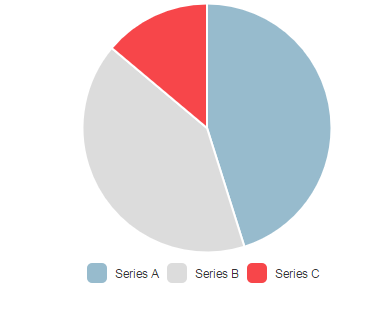
\includegraphics[width=2.5in]{chart}
%	\caption{TODO}
%	\label{sl:ma}
%\end{figure}

\section{Zaključek}
Že v sami IMapBook množici, se dva ocenjevalca pri vseh odgovorih nista strinjala o njihovi oceni. Pri ocenjevanju je računalniški algoritem lahko le tako dober kot je človek. Če se človek ne more strinjati o oceni, je težko pričakovati, da bo algoritem opravil boljše.\\

Izvorna koda je dostopna na git repozitoriju: https://github.com/TilenTomakic/IMapBooks-AQRG

Docker vsebnik s strežnikom je dostopen na spletnem naslov:
https://hub.docker.com/r/tilen/sag

\ifCLASSOPTIONcaptionsoff
  \newpage
\fi

% literature (use BibTeX)
\bibliographystyle{IEEEtran}
\bibliography{literatura}

\end{document}
